\chapter{Introduction}
The economies of \textit{all} developed nations are dependent on software. More and more systems are software controlled. Expenditure on software represents a significant fraction of GNP\footnote{General National Product.} in all developed countries.

Globally, the ICT Market is growing up every year. In 2014 the GNP due to ICT market was about 3 times of the one generated by the Automotive market.

\section{Definitions and concepts}
\textbf{Software} is a collection of computer programs, procedures, rules, associated documentation and data.
\begin{itemize}
\item Software development is more than merely the development of programs;
\item Software includes documents describing various views for various stakeholders (e.g.,\@ users, developers).
\end{itemize}
For a given problem, software is approximately 10 times more expensive to produce than a simple program (on average, 10 to 50 LoC\footnote{Line of Codes.} per person day, about 7 LoC in critical systems).

\paragraph{Types of software}
\begin{itemize}
\item Standalone;
\item Embedded: The software is a portion of the entire system;
\item Process support: Process automation, user actions are supported by software.
\end{itemize}

\paragraph{Criticality levels}
\begin{itemize}
\item Safety critical: risk of life losses (aerospace, military, medical, \dots);
\item Mission critical: risk of money loss (banking, logistics, industrial production, \dots);
\item Other: Games, \dots
\end{itemize}

\paragraph{Complexity}
\emph{Complexity} is the number of parts and interactions among parts. Software systems are probably the most complex human artifacts.

\paragraph{Diffusion}
Until 80's software was developed only for specific purposes in large private organizations, military field, banks \dots

Today software impacts on everyday's life, because of the huge diffusion of computing and ``free'' hardware.

\paragraph{Typical software problems}
\begin{itemize}
\item Too expensive (up to a factor of 10);
\item Delivered too late (up to a factor of 2);
\item Does not live up to user expectations.
\end{itemize}

\section{Misconceptions}
\paragraph{Software is free} Software requires intensive tasks and it is the dominant part in development cost.

\begin{figure}[hbtp]
\centering
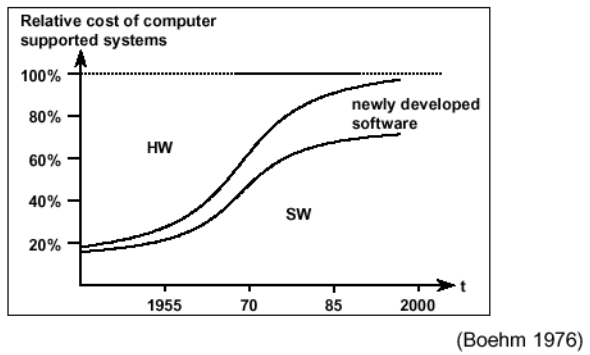
\includegraphics[scale=0.4]{images/software_cost.png}
\caption{Sofware cost}
\end{figure}

\paragraph{Software is soft} Changing software is difficult and costly. In fact, \emph{maintenance} is more expensive than development and it becomes impossible at a certain point, even if a software that is used needs continuous changing.

\paragraph{Software is produced} Software is not mass produced and replication is almost effortless. In fact, software is the product of a development process which is a non-deterministic and creative process due to human involvement. There are no timing and cost estimations and the quality is not valuable in advance.

\paragraph{Software ages} Software does not break as it ages. In fact, failures do not occur due to material fatigue (as with hardware) but due to the execution of logical faults.

Software cannot be perfect, because it is impossible to remove all software faults before execution.

Software is not stable, because it changes according to requirements changes, platform changes, and defect corrections.

\section{Product \& process}
There is no way to prove that a software product is correct because it is impossible to test it completely. In fact, a complete test requires too much time.

\paragraph{Process properties}
\begin{itemize}
\item Cost;
\item Effort;
\item Punctuality.
\end{itemize}

\paragraph{Product properties}
\begin{itemize}
\item Functionality: set of functions that satisfy stated or implied needs;
\item Correctness: capability to provide the intended functionality in \emph{all} cases;
\item Reliability: ability to perform its required functions under stated conditions for a specified period of time;
\item Safety: capability of avoiding hazards;\item Performance:
\begin{itemize}
\item Time: speed/delay to perform a function;
\item Space: memory required to perform a function.
\end{itemize}
\item Robustness: capability of providing a reduced functionality in adverse (non nominal) conditions, i.e.,\@ emergency mode);
\item Usability: ease of use of a function \begin{itemize}
\item Effort needed to use the product;
\item Assessment by the user about using the product.
\end{itemize}
\end{itemize}

\section{Software engineering}
\emph{Software engineering} is very different from ``solo programming''. In fact it is defined as multiperson construction of multiversion software\footnote{Parnas.}. \emph{Multiperson} because it involves several teams and \emph{multiversion} because it is possible to identify different versions of the software tracking changes.

Software engineering includes principles, techniques and methods to guide the development and maintenance of software with defined process and product attributes.

\begin{center}
\begin{tabular}{l|p{0.25\textwidth}l}
\toprule
&	Solo programming	&	Software engineering	\\
\midrule
Size	&	Small	&	Large \\
User	&	Developer	&	Not the developer	\\
Lifespan	&	Short	&	Long (no ageing) \\
Cost	&	Limited	&	Development + operation/maintenance \\
Properties	&	Functional	& Functional and not functional	\\
\bottomrule
\end{tabular}
\end{center}

\subsection{Principles}
Fundamental, broad coverage ideas, capable of producing positive, useful effects.

\paragraph{Separation of concerns}
Given a large, difficult problem, try to split in many independent parts and consider a single part a time. Software process must concentrate on what the system should do, then on how, and finally do it.

\paragraph{Abstraction}
Given a difficult problem/system, extract a simpler view of it, avoiding unneeded details and reason on the \textbf{model}.

\paragraph{Modularity}
Divide a complex system in modules, with \emph{high cohesion}\footnote{Many links within the same module.} and \emph{low coupling}\footnote{A few links among different modules.}. In complex systems, each module should hide to others as many details, about its internal mechanism/design choices, as possible.

\subsection{Issues}
\begin{itemize}
\item Team based development: rules and tools are required for communication and coordination between team members and among teams;
\item Long lifespan: different teams for development and maintenance. Documentation is needed;
\item Third party requirements: collecting requirements and non functional properties from a non-computer specialist.
\end{itemize}

\paragraph{Functional vs. non functional requirements}
Functional requirements are easy to express and to identify. Non functional requirements, instead, are more difficult to express and to design. They are \emph{emerging properties}, so they depend on the whole system, not only on a specific part (i.e.,\@ user experience, reliability, performance, space and time efficiency, \dots).